\documentclass[12pt,a4paper]{article} 
\usepackage[portuguese]{babel}
\usepackage[utf8]{inputenc}
\usepackage{adjustbox}
\usepackage{amsmath} 
\usepackage{graphicx}
\usepackage{booktabs}
\usepackage{float}
\begin{document}
\setcounter{figure}{4}
\setcounter{section}{3}
\setcounter{page}{5}
\section{Relatório}
\subsection{Introdução}
A maior aplicação do diodo Zener reside na regulação de tensão de saída de fontes de alimentação. Através da utilização do diodo Zener, em conjunto com um resistor, pode-se conseguir que uma fonte de alimentação forneça tensão praticamente constante à carga. O comportamento do diodo Zener na região de ruptura permite a montagem de circuitos reguladores de tensão, que serão extremamente utéis para a fontes de corrente contínua, a fim de reduzir o fator de ripple destas, assim como ilustrado na Figura~\ref{fig:esquema_tensao}.

\begin{figure}[htpb]
  \centering
  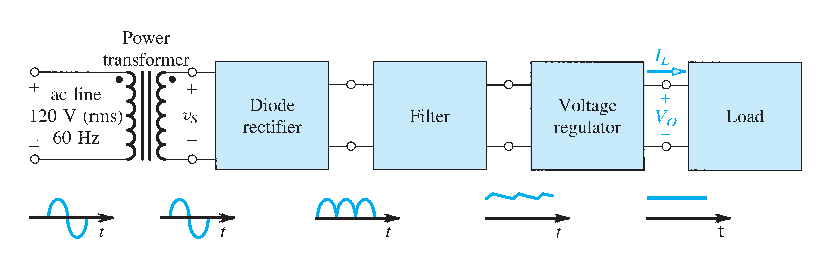
\includegraphics[width=0.8\linewidth]{./blocotransformador.pdf}
  \caption{Diagrama de blocos de uma fonte \emph{DC}.}
  \label{fig:esquema_tensao}
\end{figure}
A Figura~\ref{fig:breakdown} nos mostra detalhes da operação do diodo na região de ruptura. Observamos a existência de uma resistência dinâmica, $r_z$, o que implicará que a tensão que será aplicada na carga, $V_o$, terá uma pequena dependência na fonte de tensão, $V_s$. Em outras palavras, esperamos que se $V_s$ aumente, $V_o$ também será acrescido de um pequeno valor. O parâmetro que relaciona a variação de $V_o$ e de $V_s$ é chamado de regulação de linha.

Usando o raciocínio análogo ao parágrafo anterior, podemos relacionar a variação na  corrente da carga e na tensão de saída, dado que temos uma resistência dinâmica $r_z$. No entanto, também há a possibilidade de pensarmos em termos de resistência, já que $i_l= \frac{V_o}{R_l}$. Logo, teremos uma pequena dependência entre a resistência da carga, $R_l$, e a tensão da carga $V_o$. O parâmetro que relaciona a variação de $V-o$ e $i_l$ é chamado de regulação de carga. 

Neste experimento, estudaremos ambos os parâmetros e ainda exploraremos um componente mais sofisticado para regulagem de tensão, um circuito integrado da família $78xx$. O circuito integrado $7805$ é um regulador linear de tensão, e será utilizado em diversas configurações, cada qual com sua própria aplicação. Um regulador linear tensão, garante que se a tensão é garantidamente maior que um certo valor, um outro valor, mais baixo, será dado como saída.

\begin{figure}[htpb]
  \centering
  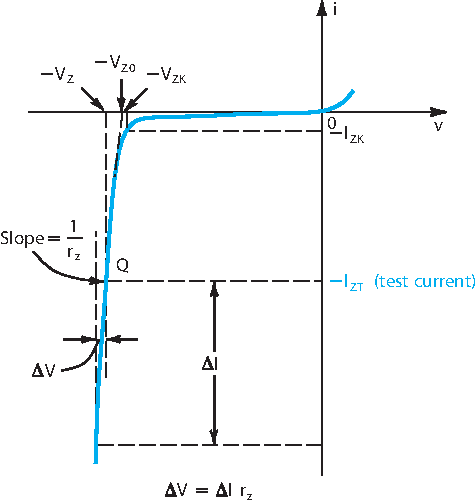
\includegraphics[width=0.6\linewidth]{breakdown_region.pdf}
  \caption{Relação detalhada da corrente e tensão de um Diodo Zener operando na região de ruptura.}
  \label{fig:breakdown}
\end{figure}

\newpage
\subsection{Análises}
%Exp1

No experimento de número 1, montou-se o circuito descrito pela Figura~1, e nos terminais do capacitor, obtivemos a Figura~\ref{entrada_exp1} através de um osciloscópio. Para $V_{i}$, constatou-se os seguintes valores:
\begin{align*}
V_{medio} = 19.3 V \\
V_{rms} = 140 mV \\
V_{min} = 19.1 V \\
V_{max} = 19.7 V 
\end{align*}

De forma semelhante, observamos o comportamento da tensão $V_o$ nos terminais da carga, obtendo assim a Figura~\ref{saida_exp1}. \\ As medidas relevantes para $V_{o}$ foram:
\begin{align*}
V_{medio} = 8.6 V \\
V_{rms} = 140 mV \\
V_{min} = 8.4 V \\
V_{max} = 8.8 V 
\end{align*}

Notou-se que os sinais, quando visualizados na tela do osciloscópio, parecem estar perfeitamente constantes. No entanto, quando coletados e graficados os dados deste sinal,  observou-se pequenas flutuações entre os valores. Ressalta-se aqui, a importância da coleta de dados.

\begin{figure}[htpb]
  \centering
  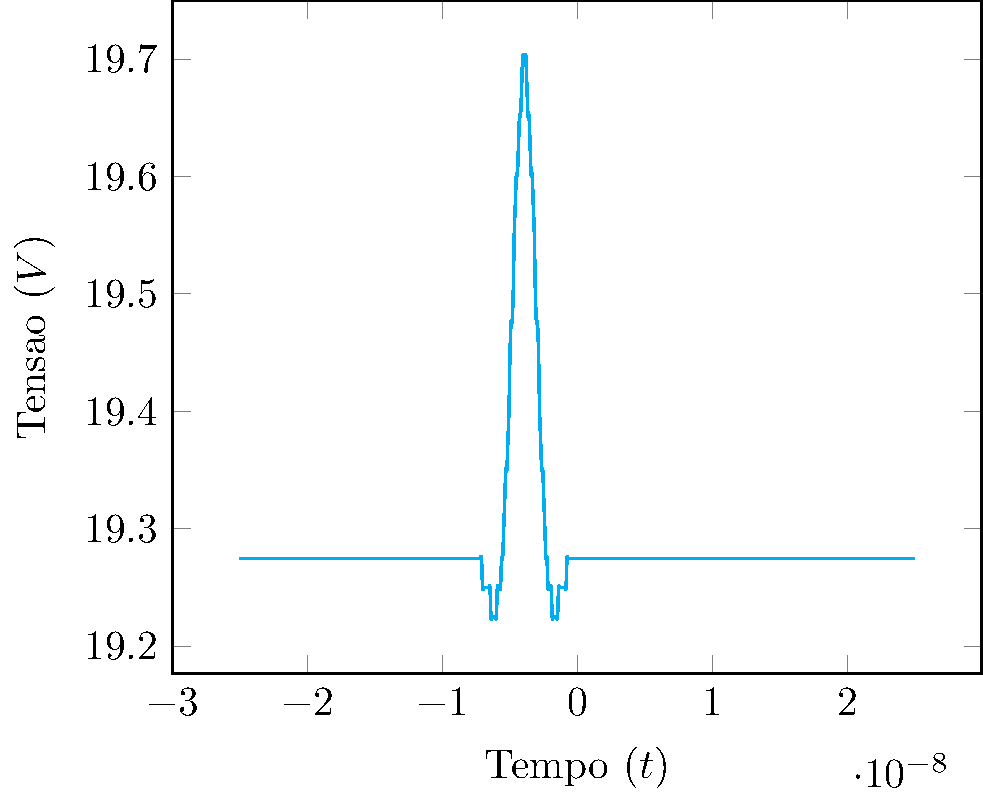
\includegraphics[width=0.8\linewidth]{./exp1/entrada_exp1.pdf}
  \caption{Sinal de entrada do circuito descrito na Figura~1, $V_{i}$, medida nos terminais do capacitor $C_1$ .}
  \label{entrada_exp1}
\end{figure}
\begin{figure}[htpb]
  \centering
  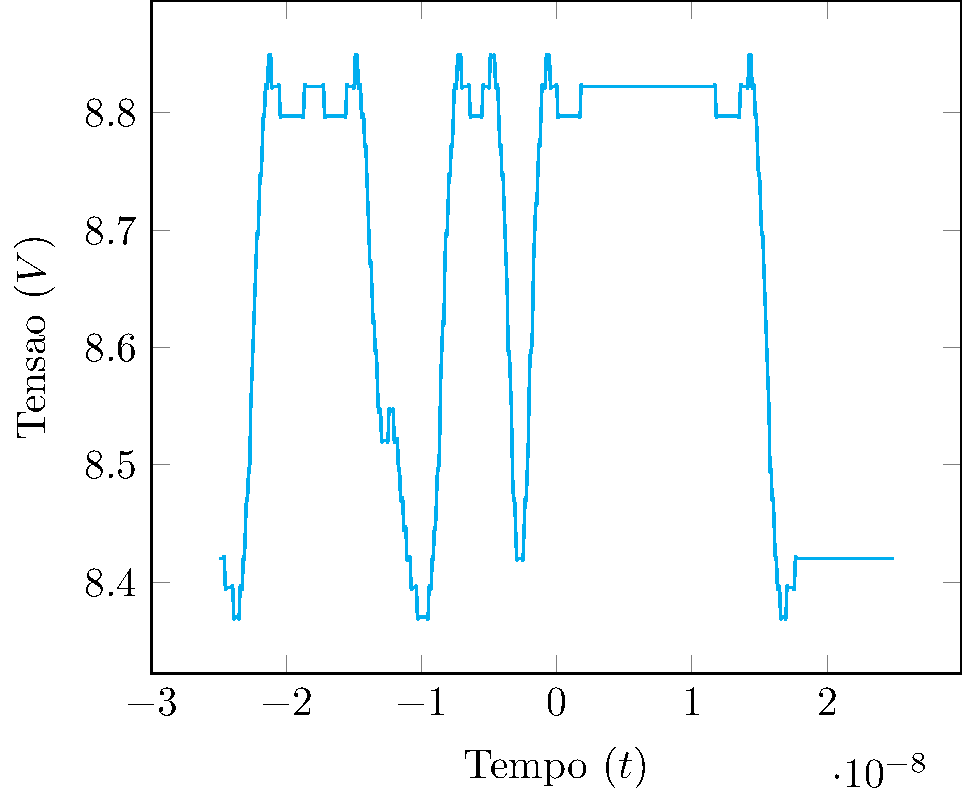
\includegraphics[width=0.8\linewidth]{./exp1/saida_exp1.pdf}

  \caption{Sinal de saída do circuito descrito na Figura~1, $V_{o}$, medida nos terminais da carga $R_l$ .}
  \label{saida_exp1}
\end{figure}
%exp2

No experimento de número 2, montou-se o circuito descrito pela Figura~2, e nos terminais do capacitor, obtivemos a Figura~\ref{entrada_exp2} através de um osciloscópio. Para $V_{i}$, constatou-se os seguintes valores:
\begin{align*}
V_{medio} = 19.5 V \\
V_{rms} = 90mV \\
V_{min} = 19.2 V \\
V_{max} = 19.7 V 
\end{align*}

De forma semelhante, observamos o comportamento da tensão $V_o$ nos terminais da carga, obtendo assim a Figura~\ref{saida_exp2}. \\ As medidas relevantes para $V_{o}$ foram:
\begin{align*}
V_{medio} = 4.4 V \\
V_{rms} = 60 mV \\
V_{min} = 4.4 V \\
V_{max} = 4.8 V 
\end{align*}

\begin{figure}[htpb]
  \centering
  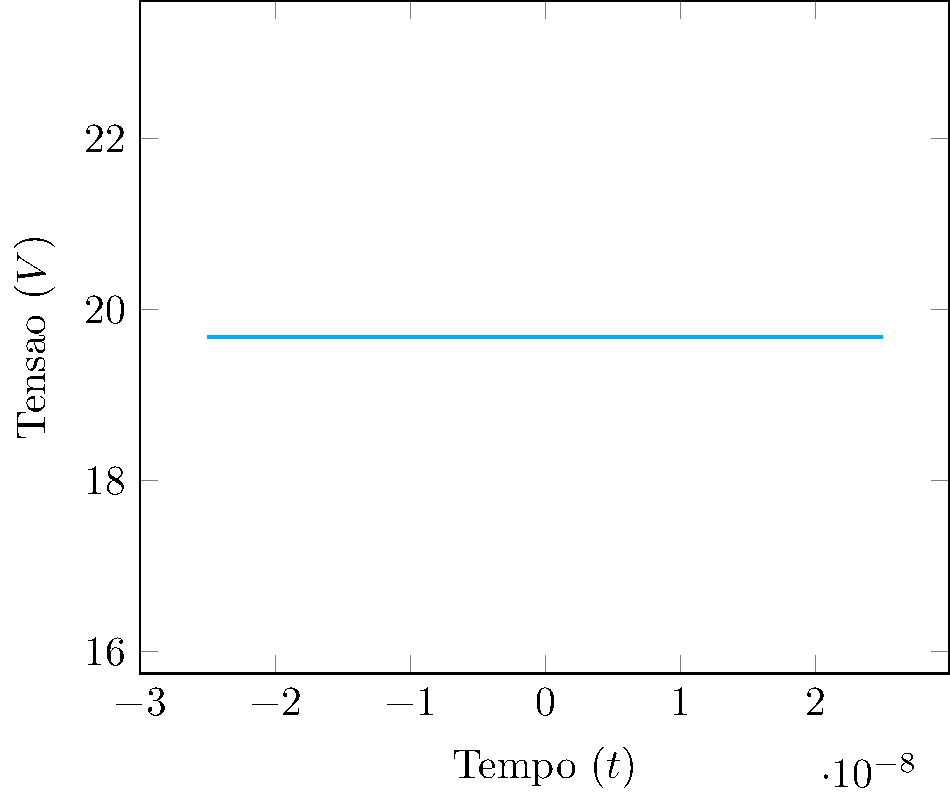
\includegraphics[width=0.8\linewidth]{./exp2/entrada_exp2.pdf}
  \caption{Sinal de entrada do circuito descrito na Figura~2, $V_{i}$, medida nos terminais do capacitor $C_1$ .}
  \label{entrada_exp2}
\end{figure}
\begin{figure}[htpb]
  \centering
  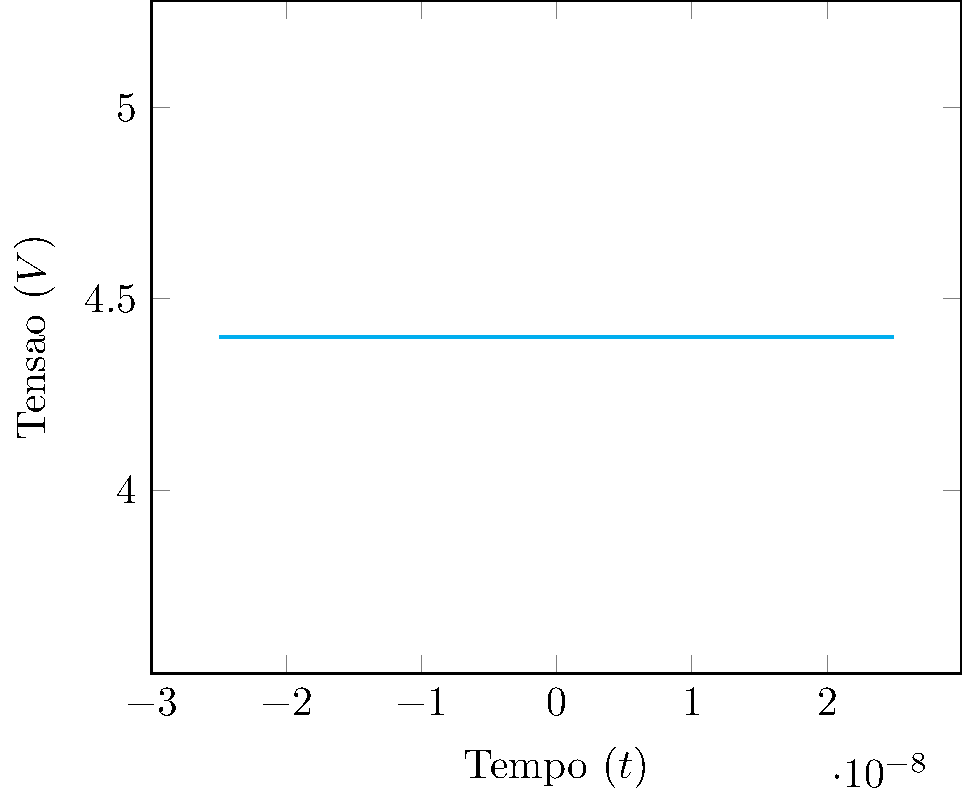
\includegraphics[width=0.8\linewidth]{./exp2/saida_exp2.pdf}
  \caption{Sinal de saída do circuito descrito na Figura~2, $V_{o}$, medida nos terminais da carga $R_l$ .}
  \label{saida_exp2}
\end{figure}
%exp3 

No experimento de número 3, montou-se o circuito descrito pela Figura~3, e variando o potenciômetro, percebeu-se a influência da variação de carga no circuito. Para uma medida mais precisa, representou-se o potenciômetro por 3 resistências e obteu-se a Tabela~\ref{exp3}.

\begin{table}[htpb]
  \centering
  \caption{Valores obtidos através do osciloscópio para três diferentes resistências, paralelas com a carga, no sistema descrito pela Figura~3.}
  \label{exp3}
  \begin{tabular}{c c c c}
    \toprule
    $[\Omega]$ & Médio $[V]$ & Mínimo $[V]$  &  Máximo $[V]$\\ \midrule
   100  & $320 \times 10^{-3}$ & $200 \times 10^{-3}$& $400 \times 10^{-3}$ \\\midrule
   470& 2.3& 2.2& 2.4 \\\midrule
   820& 4.15& 4& 4.2 \\ \bottomrule 
  \end{tabular}
\end{table}
%exp4

No experimento de número 4, montou-se o circuito descrito pela Figura~4, e utilizou-se de um amperímetro para medir a corrente em $R_l$ e de um voltímetro para medir $V_o$. Repetindo a medição para dois valores de resistência distintos, construi-se a Tabela~\ref{exp4}. 
\begin{table}[htpb]
  \centering
  \caption{Valores obtidos através de um voltímetro e um amperímetro para duas diferentes cargas no sistema descrito pela Figura~4.}
  \label{exp4}
  \begin{tabular}{c c c }
    \toprule
    $[\Omega]$ & $V_{l} [V]$&$i_l [mA]$  \\ \midrule
   47& 20.35& 111.5 \\\midrule
   100& 2.3& 56.1 \\\midrule
  \end{tabular}
\end{table}

\newpage
\subsection{Discussões}
O diodo Zener, quando reversamente polarizado em uma tensão suficiente para que se atinja a zona de ruptura,  se comporta como um regulador de tensão, que proporcionará uma queda de tensão constante, no caso $8.8 V$. Como o diodo Zener está em paralelo com a carga, esta sofrerá uma queda constante de mesmo valor. O resistor $R_s$ é responsável por controlar a quantidade de corrente que entrará no diodo Zener e na carga, pois a queda de tensão nele será $V_{i}-V_{z}$, sendo $V_{z}$ a tensão no terminal do diodo Zener. Nota-se aqui, que o fator de ondulação é muito próximo de zero, pois a tensão saída é praticamente constante.

Para uma configuração em que se manteve fixo $V_i$ e $R_l$ variável, determinou-se os limites de operação do regulador Zener, utilizando-se, quando necessário, as informações do datasheet (Fairchild Nov-2014) presentes na Tabela~\ref{data_1n4007}.
\begin{table}[htpb]
  \centering
  \caption{Datasheet do 1N4007 retirado da fabricante Fairchild (Novembro de 2014).}
  \label{data_1n4007}
  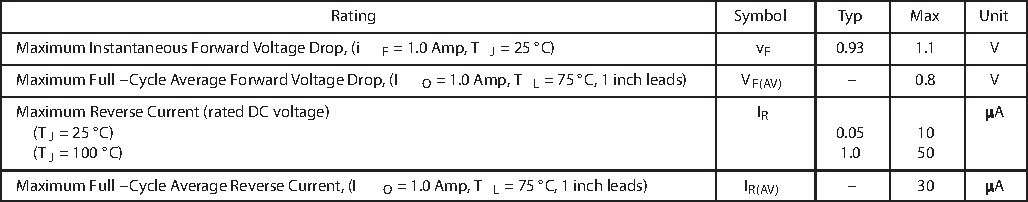
\includegraphics[width=\linewidth]{1n4007.pdf}
\end{table}
\begin{align}
  R_{L_{min} }=&  \frac{R V_{z}}{V_i - V_{z}}\\ \nonumber
  R_{L_{min} }=&  \frac{820 \times 8.8}{19.3-8.8} = 687.24 \Omega 
\end{align}
\begin{align}
  I_{L_{max} }=&  \frac{V_{z}}{R_{l_{min}}}\\ \nonumber
  I_{L_{max} }=&  \frac{8.8}{687.24} = 12.8 mA
\end{align}
\begin{align}
  I_{R}=&  \frac{V_{R}}{R}\\ \nonumber
  I_{R}=&  \frac{8.5}{820}= 10.73 mA
\end{align}
\begin{align}
  I_{L_{min} }=&  I_R - I_{zm}\\\nonumber
  I_{L_{min} }=&  10.73 \times 10^{-3}- 30 \times 10^{-6}= 10.7 mA 
\end{align}
\begin{align}
  R_{l_{max}} =&\frac{V_{z}}{I_{l_{min}}} \\ \nonumber
  R_{l_{max}} =&\frac{8.8}{10.7 \times 10^{-3}} = 822.43 \Omega 
\end{align}

Para o experimento 2, temos o valor máximo de corrente de carga quando toda corrente passar apenas pela carga. Para uma tensão $V_{max}=4.8 V$ e uma carga fixa de $1 k\Omega$, teremos uma corrente máxima na carga $I_{l_{max}}=4.8 mA$. Utilizando-se parte do datasheet (Fairchild Sep 2014) da família \emph{78xx/78xxA}, a tensão de entrada mínima é $7V$.

Para o circuito do experimento 3, obteu-se a expressão de $V_o$ em função de $R_1$ e $R_2$ e na corrente do terminal 2 do regulador de tensão $7805$. Para os cálculos utilizou-se da informação que a diferença de tensão entre o pino 2 (\emph{GND}) e o pino 3 (\emph{Output}) é de $5V (4.8-5.2V)$ segundo o datasheet mostrado na Tabela~\ref{data_7805}. 
\begin{table}[htpb]
  \centering
  \caption{Datasheet do 7805 retirado da fabricante Fairchild (Setembro de 2014).}
  \label{data_7805}
  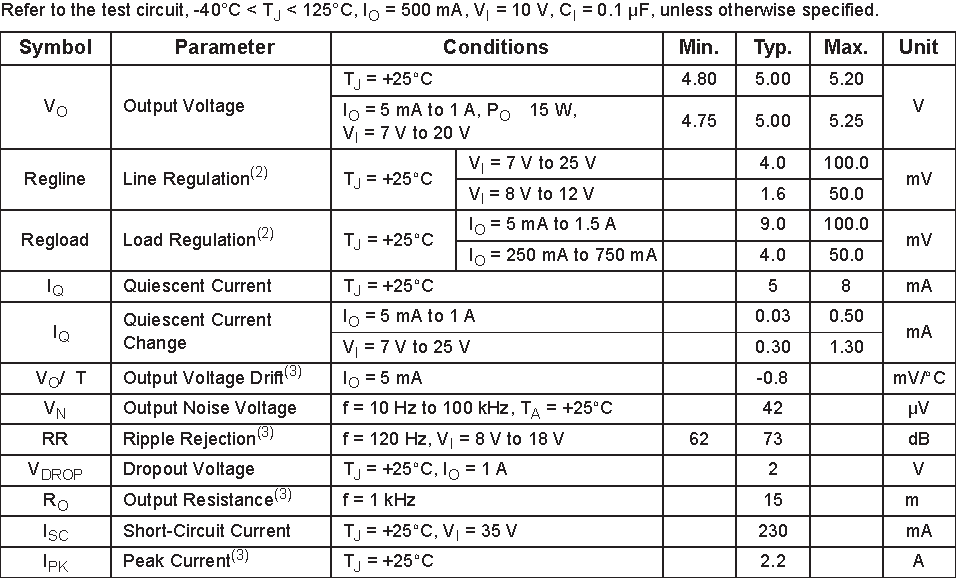
\includegraphics[width=\linewidth]{7805.pdf}
\end{table}

\begin{align}
  V_o \frac{R_2 }{R_1+R_2} = V_o -5 \\ \nonumber
  V_o \left(\frac{R_2 }{R_1+R_2} -1 \right) =-5 \\\nonumber
  V_o= \frac{5}{R_1} \left(R_2 +R_1\right)\\\nonumber
  V_o= I_2 \left(R_2 +R_1\right)\nonumber
\end{align}
Para o valor mínimo do potenciômetro de $100\Omega$ calculou-se:
\begin{align*}
  V_o = 0.01 \times \left( 100+470 \right)= 5.7 V
\end{align*}

\newpage
\subsection{Conclusão} \end{document}
